\documentclass[a4paper]{article}
\usepackage[utf8]{inputenc}
\usepackage[english]{babel}
\usepackage[hidelinks]{hyperref}
\usepackage{graphicx}
\usepackage[table]{xcolor}
\usepackage{color}
\usepackage{caption}
\usepackage{subcaption}
\usepackage{pdfpages}
\usepackage[nottoc,numbib]{tocbibind} 
\usepackage{mathpartir}
\usepackage{mathtools}
\usepackage{listings}
\usepackage{xcolor}
\usepackage{pdfpages}
\usepackage{amssymb}
\lstset { 
	language=C++,
	%backgroundcolor=\color{black!5}, % set backgroundcolor
	basicstyle=\footnotesize,% basic font setting
	%numbers=left
}

%Commands
\newcommand{\source}[1]{\caption*{Source: {#1}} }
\newcommand{\qs}{\texttt{QuadSketch}}
\newcommand{\qt}{\textit{Quad Tree}}
\newcommand{\qsr}{\texttt{QSR}}
\newcommand{\grid}{\texttt{Grid}}
\newcommand{\tm}[1]{\textit{Theorem {#1}}}
\newcommand{\bo}[1]{$\mathcal{O}$(\textit{#1)}}
\newcommand{\bos}[1]{$\mathcal{\text{Õ}}$(\textit{#1)}}
\newcommand{\pq}{\texttt{PQ}}
\newcommand{\gr}{\texttt{Grid}}
\newcommand{\mnist}{\texttt{MNIST}}
\newcommand{\sift}{\texttt{SIFT}}
\newcommand{\clust}{\texttt{CLUSTERS}}
\newcommand{\gist}{\texttt{GIST}}




\begin{document}
\pagenumbering{gobble} %remove page numbering
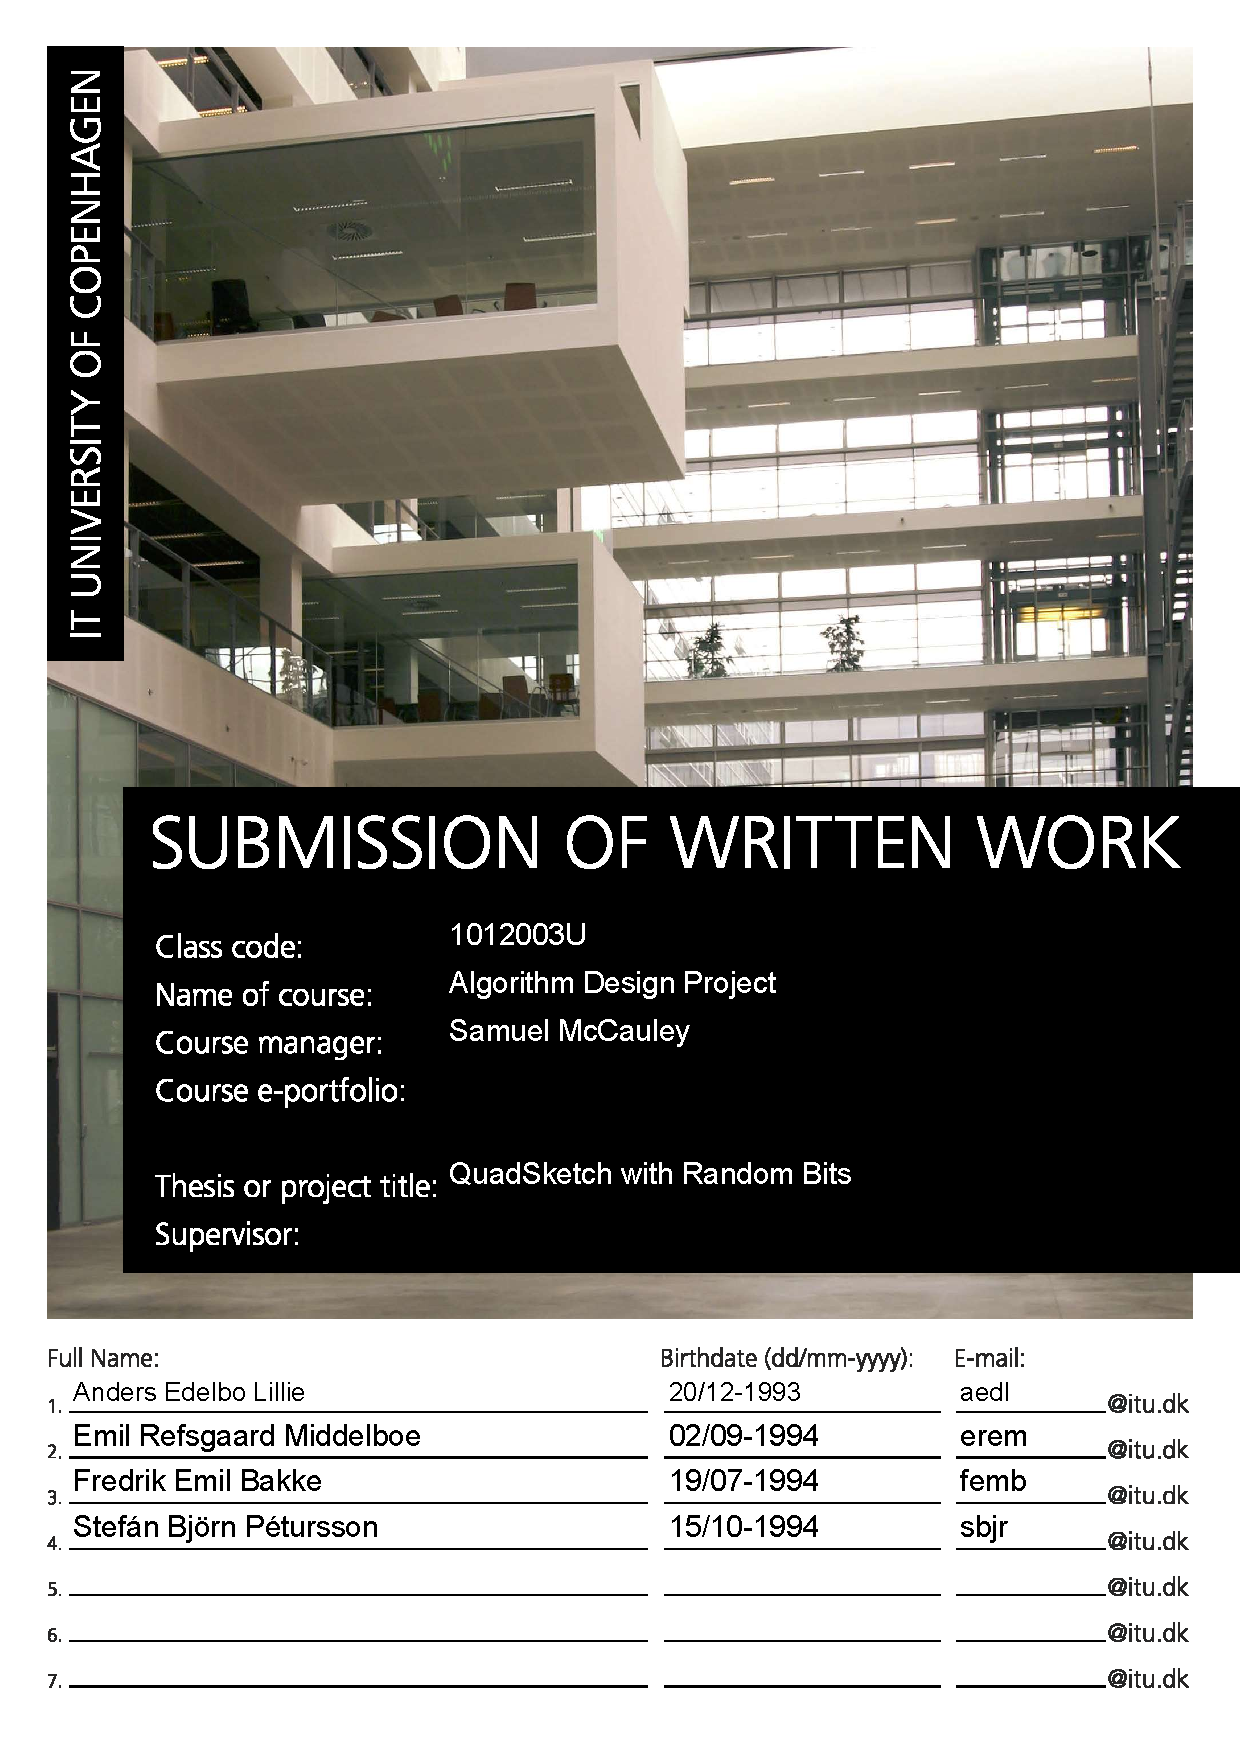
\includepdf[pages=-]{frontpage.pdf}
\begin{titlepage}
	
	\newcommand{\HRule}{\rule{\linewidth}{0.5mm}} % Defines a new command for the horizontal lines, change thickness here
	
	\center % Center everything on the page
	
	\textsc{\LARGE IT University of Copenhagen}\\[1.5cm] % Name of univerEFsity
	\textsc{\Large Software Development MSc}\\[0.5cm] % Major heading
	\textsc{\large Algorithm Design Project}\\[0.5cm] % Minor heading
	
	\HRule \\[0.4cm]
	{ \huge \bfseries QuadSketch with Random Bits}\\[0.4cm] % Title of document
	\HRule \\[1.5cm]
	
	\begin{minipage}{0.5\textwidth}
		\begin{flushleft} \large
			\emph{Authors:}\\
			Anders Edelbo \textsc{Lillie} \\
			Emil Refsgaard \textsc{Middelboe} \\
			Fredrik Emil \textsc{Bakke} \\
			Stefán Björn \textsc{Pétursson}
		\end{flushleft}
	\end{minipage}
	~
	\begin{minipage}{0.4\textwidth}
		\begin{flushright} \large
			\emph{Supervisors:} \\
			Samuel \textsc{McCauley} \\
			Johan von Tangen \textsc{Sivertsen}
		\end{flushright}
	\end{minipage}\\[4cm]
	
	{\large \today}\\[3cm] 
	
	\vfill % Fill the rest of the page with whitespace
	
\end{titlepage}

\begin{abstract}
This paper analyzes, experiment, and verifies the relatively new algorithm \qs{} proposed in \cite{wagner17} and makes a contribution by modifying the pruning/decompression step of \qs{}. A baseline algorithm has been implemented to properly verify the experiments and results from \cite{wagner17}, and shows \qs{} outperforms the baseline algorithm as presented in \cite{wagner17}. Experiments compared the performance of \qs{} against the modified algorithm \qsr{}. The experiments showed a better average case performance of \qsr{} in regards to accuracy and distortion over \qs{}. Furthermore there is given a theoretical proof of \qsr{} giving a better expected distance perseverance than \qs{}. 
  \dots Furthermore \qs{} has been tested on a new type of data set, "NAME", which reveals that \dots
\end{abstract}
\clearpage

\tableofcontents
\clearpage
\pagenumbering{arabic} %reset page numbering
	
%sections
\section{Introduction}
\label{introduction}
%Formal introduction goes here

\subsection{Motivation} %Why are we interested in this?

\subsection{Case} %What is the QuadSketch paper about?

\subsection{Problem definition} %What is our research question?
%From ILO:
%"Plan and carry out a small-scale investigation of an algorithmic research problem. This investigation could be theoretical, experimental, or both."

\section{Contribution}
\label{contribution}
%Short section about our final findings and contributions
%This section describes the contributions given to \qs{} as the results for this project.
This section will briefly present the results of the project\footnote{See \url{https://github.com/aelillie/quadsketch} for the GitHub repository for the project}. Through experiments on SIFT and MNIST with the \qs{} implementation, as well as a version of \gr{} it is observed that the results are comparable to those reported in \cite{wagner17}. 

Furthermore an extension of \qs{} called \qsr{} (for QuadSketch Random) is implemented, where the decompression step has been modified. Instead of placing zeros in the bit representation of a point, which is deemed "non-important" to the compression scheme(called \textit{long edges} in the paper), bits are inserted at random. Empirical experiments show slight improvements from \qsr{} over \qs{}. The most significant of which is for the experiments on the \mnist{} dataset, where \qsr{} overall performs better than \qs{}. The average result reached for each block size in the tests are summarized in tables \ref{table:avg_mnist_qs1} and \ref{table:avg_mnist_qsr1}, where high accuracy and low distortion with minimum size is better. Note however that the implemented modification does not alter the sketch size, which is influenced by other factors. Even though the algorithm in its core is highly influenced by some randomness(see section \ref{qs}), the results gained from the experiments are quite convincing. In section \ref{results}, this is further demonstrated in figure \ref{fig:graph mnist}, which visualizes the test results in a graph. Additionally an expected performance gain is obtained by the fact that random bit insertion ensures a lower distortion of pruned points, it is presented in section \ref{exp:dist}.

%TODO: Insert probability or distance improvements with QSR

\begin{table}[h]
	\centering
	\caption{Average Results for \qs{} on \mnist{}}
	\label{table:avg_mnist_qs1}
	\begin{tabular}{l l l l}
		\hline
		\#Blocks & Bits per coordinate & Accuracy  & Distortion \\ \hline
		2 & 3.43 & 0.44 & 1.100  \\
		4 & 4.36 & 0.51 & 1.096  \\
		7 & 3.75 & 0.53 & 1.097 \\
		8 & 3.69 & 0.56 & 1.09 \\
		14 & 3.51 & 0.67 & 1.048 \\
		16 & 3.45 & 0.69 & 1.039 \\
		28 & 3.35 & 0.81 & 1.013 \\
		\hline
	\end{tabular}
\end{table}

\begin{table}[h]
	\centering
	\caption{Average Results for \qsr{} on  \mnist{}}
	\label{table:avg_mnist_qsr1}
	\begin{tabular}{l l l l}
		\hline
		\#Blocks & Bits per coordinate & Accuracy  & Distortion \\ \hline
		2 & 3.79 & 0.55 & 1.118  \\
		4 & 3.73 & 0.57 & 1.09  \\
		7 & 3.21 & 0.62 & 1.062 \\
		8 & 3.16 & 0.64 & 1.052 \\
		14 & 3.01 & 0.74 & 1.023 \\
		16 & 2.95 & 0.76 & 1.02 \\
		28 & 2.87 & 0.85 & 1.008 \\
		\hline
	\end{tabular}
\end{table}

\section{Background}
\label{background}
This section will present relevant background information for reading this paper, including the research area in section \ref{research_area}, the \qs{} algorithm in \ref{qs}, and related work in \ref{state_of_the_art}.

\subsection{Research area}
\label{research_area}
%What is the research area?
Various algorithms exist to find distances between data points in a (typically large) data set. One example is doing similarity search, or more specifically ANN search, on pictures to recognize letters or numbers. As useful as this is, it still depends on the given data, which is getting increasingly big in size and suffers from the \textit{curse of dimensionality}. This is a general problem as even modern machines are not able to process \textit{gigantic} files all at once(i.e. keeping all the data in main memory). Thus another big subject in computer science arises, that is compressing the data in order to fit it in memory while trying to preserve relevant properties from the data. One particular scheme is referred to as \textit{quantization}, which is the process of constraining an input from a continuous set of values to a discrete set\footnote{E.g. real numbers to integers. See https://en.wikipedia.org/wiki/Quantization 11-04-2018}. This research area is what \qs{} deals with, and in particular for high-dimensional data sets. 
\\
\\
Naturally one must pay to compress something, which happens in terms of accuracy, i.e. representing the data using only approximations. This also means there is a trade off between compression and accuracy for the algorithms in this area. Compression algorithms are usually measured on these parameters, i.e. accuracy per compression size\cite{wagner17,schmid9}.
\\
\\
Distance preserving compression algorithms are usually divided into two categories: data-oblivious and data-dependent. The former attempts to achieve guarantees for any data set while the latter attempts to use the extra information about the particular data sets in order to design functions with better performance. Compressed representations makes computation for data analysis algorithms more efficient, which is very desirable in many fields, such as data mining and machine learning\cite{stan15}.

\subsection{The \qs{} compression scheme}
\label{qs}
In this section the \qs{} algorithm is outlined. The compression scheme that it comprises produces a sketch, which is a compressed representation of a point set \texttt{X}. The points of \texttt{X} have \texttt{d} dimensions and are in \textit{Euclidean} space. Each coordinate of a point is represented by \texttt{B} bits implying that a point is represented by \textit{dB} bits. \qs{} requires the point set \texttt{X} and two additional parameters, namely \texttt{L} and $\Lambda$ as input. These two parameters are used to specify the compression of the point set where \texttt{L} is the depth of the \qt{} and $\Lambda$ controls the amount of nodes from \qt{} which can be pruned. Furthermore a number of \textit{blocks} is required to run the extended algorithm presented in \tm{3}(see below).

There are three steps for building the sketch: randomly shifted grid, \qt{} construction and pruning. These steps will be explained briefly and a small example of how a \qt{} is built and pruned will be given.
\\
\\
The first step is to produce a randomly shifted grid on the hypercube(an n-dimensional space) \texttt{H} which contains all points of the given point set \texttt{X}. \texttt{H} will then be set up to be centered around a point of \texttt{X}. Then a random value, $\sigma_j$, is chosen for each dimension \texttt{j} to shift \texttt{H}. This results in a randomly shifted axis-parallel grid on the points. It is however noted in the paper that this step often can be eliminated in practice without affecting the empirical performance of the algorithm, but that it is necessary for achieving guarantees for arbitrary point sets\cite[p. 4, "Step 1"]{wagner17}.
\\
\\
The next step is to create the \qt{}. A \qt{} is created by starting at the root of \texttt{H}. Child nodes are only added for the corresponding grid cells that contain at least one point of \texttt{X}, and thus child nodes that do not contain a point from \texttt{X} are ignored. Each edge to a child node is labeled with a \textit{d} long bit string that represents the values split on for each dimension. This step is done recursively until the level \textit{L} is reached. An example of a constructed \qt{} is given in figure \ref{fig:quadtree}(on the left).\\

\begin{figure}
	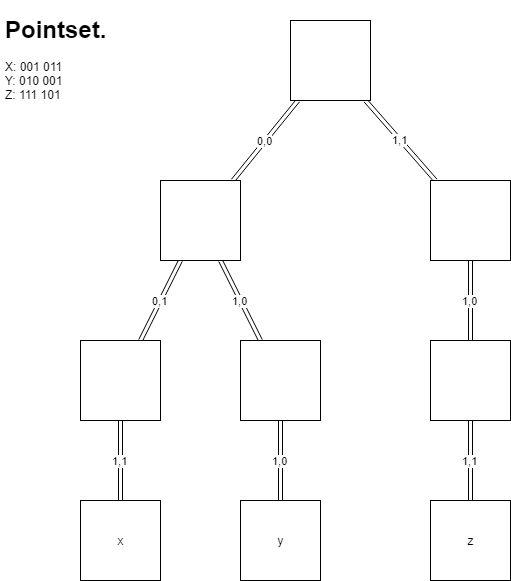
\includegraphics[width=0.5\textwidth]{figures/quadtree}
	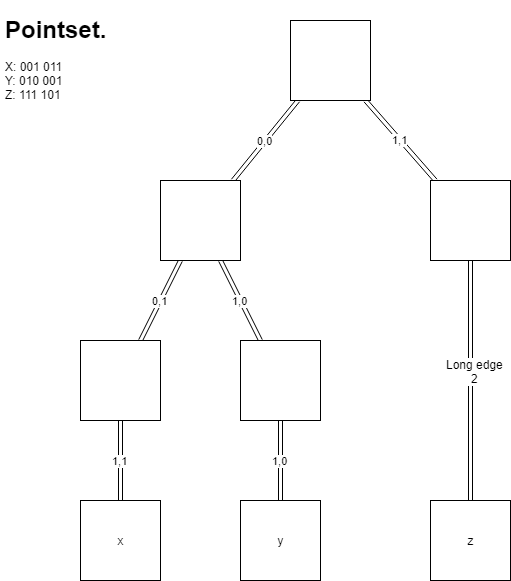
\includegraphics[width=0.5\textwidth]{figures/prunnedquadtree}
	\caption{On the left there is shown the \qt{} after construction with $L=4$. On the right the \qt{} has been pruned with a $\Lambda = 1$}
	\label{fig:quadtree}
\end{figure}

The final step is pruning. For each downward path $n_0,...,n_k$ in the \qt{} where nodes $n_1,...,n_{k-1}$ all have a degree 1, if \ensuremath{\texttt{k} > \Lambda+1} then corresponding nodes $n_{\Lambda+1},...,n_{k-1}$ are removed from the \qt{}. Instead node $n_{\Lambda}$ is connected directly to $n_{k}$ with an edge. This edge is called a \textit{long edge} and is labeled with the length of the path it replaces ($k-\Lambda$). An example of the tree after a pruning is given in figure \ref{fig:quadtree}(on the right).
\\
\\
To represent the sketch the "Eulerian Tour Technique"\footnote{See e.g., \url{https://en.wikipedia.org/wiki/Euler\_tour\_technique}} is used.
It starts at the root of the tree and searches down to the leftmost leaf. It will then backtrack up to a node from which it came and traverse down to find a new leaf in a depth first search manner. When an edge is explored downwards a 0 is stored together with the label of the edge, being either a bit string or the length of a long edge and a bit specifying if the given edge is a long or short edge. If an upwards edge is explored a 1 is stored. Furthermore an index for all the leafs are stored.
\\
\\
The paper \cite{wagner17} present three different approaches for building the previous described sketch each giving different properties for the resulting sketch. These different properties are defined as theorems, \tm{1} being the primary theorem.

\paragraph{\tm{1}} states that for each point, the distance from the given point to all other points are preserved up to a given factor $1\pm\epsilon$ with a constant probability. This is formalized as the following guarantee: for every $i\in{[n]}$
\begin{equation}
Pr[\forall{}_{j\in{}[n]} ||~x_i-~x_j||= (1\pm\epsilon)||x_i-x_j||] \geq 1 - \delta
\end{equation}
\paragraph{\tm{2}} states the property of being able to recover \textit{every} distance $||x_i-x_j||$  up to a distortion $1\pm\epsilon$ with a high probability by applying \qs{} recursively.
\paragraph{\tm{3}} is an extension of \tm{1} in which a sketch is built for $m$ blocks where a block is a subset of dimensions for the points in the dataset $X$. Here \qs{} is applied separately to each block. This gives the following guarantee, with \textit{m} added:

\begin{equation}
Pr[\forall{}_{j\in{}[n]} ||~x_i-~x_j||= (1\pm\epsilon)||x_i-x_j||] \geq 1 - m\delta
\end{equation}

%From ILO:
%"Find, extract and explain results in the algorithms research literature relevant to a given problem."
\subsection{Related work}
\label{state_of_the_art}
Due to the size of the research area, described in \ref{research_area}, a huge amount of related work to \qs{} exists. \cite{wagner17} specifically compares their algorithm to a state of the art algorithm, \textit{Product Quantization} (\pq{}), introduced in \cite{schmid9}. %Furthermore Spectral Hashing is closely relates as... Also the findings in [6] shows that...
%TODO: Write which papers are related

\subsubsection{\textit{Product Quantization}}
The \pq{} concept is stated in the abstract of the original paper as such: \textit{This paper introduces a product quantization based approach for approximate nearest neighbor search. The idea is to decompose}[..] \textit{the space into a Cartesian product of low dimensional subspaces and to quantize each subspace separately}. Specifically the algorithm uses \textit{vector quantization} as the approach to compress data, mapping a real valued vector, \textit{x}, in \textit{D}-dimensional space to \textit{centroid} representations, \textit{$c_i$}, in a set $\mathcal{V}_i$\cite[p.3 II-A]{schmid9}. The set of vectors mapped with the quantizer function \textit{q} to a given index \textit{i} is referred to as a (Voronoi) \textit{cell}, and defined as:

\begin{equation}
	\mathcal{V}_i\mathrel{\hat=}{x\in\mathbb{R}^D : q(x)=c_i}
\end{equation}

As opposed to scalar quantization, where single values are reconstructed, in this case the set of \textit{vectors}, indexed to the same cell, are reconstructed. Before applying this scheme to the vectors, the D dimensions are divided into \textit{product quantizers}, basically dividing the space into \textit{m} subvectors of \textit{D*} dimensions, such that \textit{D*$=D/m$}\cite[p.3 II-B]{schmid9}. The subvectors are then quantized seperately using \textit{m} distinct quantizers. This scheme is applied, allowing to keep very large vector codes in memory. As reference a convincing example is listed in \cite[Table I, p. 4]{schmid9}, illustrating that the k-means algorithm consumes $kD$ memory, while k-means with product quantization consumes  $k^{1/m}D$.

Besides using \pq{} as comparison algorithm in their experiments, \qs{} is actually implemented with the same idea of \textit{product quantizers}\footnote{specifically defined in \tm{3}, \cite[p. 5]{wagner17}}. \qs{} is applied to all data points for each subvector in \textit{D*} dimensions, which is referred to as \textit{blocks} in their paper. 

\subsubsection{Hashing methods} %TODO: Cite
Further algorithms on data-dependent distance preserving compression algorithms include Locality Sensitive Hashing(LSH), Semantic Hashing, and Spectral Hashing\cite{weiss8}, which all rely on hash functions for computing codes. 

The former algorithm, LSH, is popular, and widely used as reference in the research area. Instead of using a tree-like data structure, such as a kd-tree, it hashes points using several hash functions, ensuring that, for each function, the probability of collision is much higher for objects which are close to each other than for those that are far apart\footnote{It is worth noting that this is the exact opposite of what is trying to be achieved in e.g. hash tables}. Thus, one can use this scheme to hash a query point, and then retrieve near neighbors contained in the same hash bucket.

Semantic Hashing computes compact codes for data points such that the Hamming distance between two different codes are correlated with \textit{semantic similarity}(i.e. the idea of distance is based on the likeness of meaning or semantic content\footnote{\url{https://en.wikipedia.org/wiki/Semantic_similarity}. Accessed 14-05-2018}). Similar neighbors are then computed by retrieving items within a small Hamming distance from the code of the query.  

Similarly Spectral Hashing tries to obtain binary code representation of data points. This algorithm uses a bit more complex approach. It first performs a Principal component analysis (PCA) on the data, which converts it to a \textit{set of values of linearly uncorrelated variables called principal components}\footnote{\url{https://en.wikipedia.org/wiki/Principal_component_analysis}. Accessed 14-05-2018}. Then a concept of fitting a rectangular approximation along every PCA direction is performed by finding the \textit{k} smallest eigenvalues\footnote{A vector that only changes by a scalar factor when applied with a linear transformation. \url{https://en.wikipedia.org/wiki/Eigenvalues_and_eigenvectors}. Accessed 14-05-2018.}, and finally thresholding these to obtain binary codes(i.e. setting a 1 when a value is above some threshold, otherwise 0). 

\subsubsection{Near-Optimal (Euclidean) Metric Compression}
Referenced throughout \cite{wagner17} is the paper \cite{NearO}. This paper describes a method using two collaborative algorithms to construct a sketch for \textit{n} points of size \bo{nlog(1/$\epsilon$) + log log $\Phi$}, where $\Phi$ denotes the aspect ratio(see \ref{sec:aspect_ratio}). This is a lower bound than achieved by \qs{}. This method is related to \qs{} both in research area, but also in nature of the algorithms. The algorithms are based on a hierarchical clustering of the points and both uses similar pruning techniques in order to reduce the size of sketch.
\\
\\
The method described in \cite{NearO} makes use of two algorithms, namely a \textit{summation} algorithm \texttt{SUM} and an \textit{estimation} algorithm \texttt{EST}. \texttt{SUM} makes up most of the paper as this is the algortihm responsible for constructing the sketch. The \texttt{EST} algorithm is responsible for approximating the distance between two points in the sketch.

\texttt{SUM} constructs a variant of hierarchically well-separated trees (HST's) connecting each cluster C in a dataset to its related subclusters. Every node in the tree T has a mapping to their related clusters. The tree T has \textit{n} leaves and a depth up to \textit{log $\Phi$ + 2} prior to the \textit{compression} step. This compression step is quite similar to the pruning step in \cite{wagner17}, as it compresses long paths of degree-1 nodes.
\\
\\
After the compression of T, a different approach to represent the nodes than in \cite{wagner17} is used. Instead of using quantization as with \qs{}, \cite{NearO} associates three properties for each node \textit{v} $\in$ T. Firstly it associates a center, \textit{c(v)}, secondly an ingress \textit{in(v)} and thirdly a surrogate \textit{s*(v)}. %The function \textit{c(v)} points to the node which represents the center of the cluster to which \textit{v} belongs, and \textit{s*(v)} describes the approximate location of this center from \textit{v}. The \textit{in(v)} function points to another node in the same subtree as \textit{v} and is used to calculate \textit{v's} displacement from its center. 
Once these properties have been associated to each node in T, the sketch is created, storing the nodes and the structure of T, denoting long edges and short edges similarly as in \qs{}. 
\\
\\
Once the sketch has been created the method now makes use of the \texttt{EST} algorithm to produce a (1 $\pm$ $\epsilon$)-approximation for the distance between any two points in the given dataset. \texttt{EST} is able to recover the approximate surrogates related to a point, and since the surrogates exist in the same subtree as the original point. It is hence possible to deduce the approximate distance. 
%Well known general algorithms and data structures exists for the same purpose, such as \textit{k-means} and \textit{kd-trees}, where the former is a clustering algorithm and the latter is an adaptive data structure for spatial data sets. This is also discussed in \cite{schmid9}, where it is noted that apparently a pure brute-force algorithm outperforms these in practice for high-dimensional data. Further algorithms listed in this paper include "spectral hashing"\cite{weiss8}, "Hamming embedding"\cite{jegou8}, and "FLANN"\cite{muja9}. These will not be investigated further, but are only mentioned for reference.
%TODO: Elaborate on closely related work and insert citations
\section{Analysis}
\label{analysis}
%Our analysis of the paper and algorithm goes here
%From the course's intended learning outcomes (ILO):
%"Find, extract and explain results in the algorithms research literature relevant to a given problem"
%"Theoretically analyze the performance of a given algorithmic solution"
This section provides an analysis of properties of the \qs{} algorithm as introduced in \cite{wagner17}, which are deemed interesting and relevant for understanding the algorithm, and thus extend it with an improvement.

%TODO: Do we have more analysis?

\subsection{Why randomly shift hypercube?}
Randomly shifting a hypercube in each dimension is necessary for the \qs{} implementation to maintain guarantees on arbitrary datasets. A good result for the cube would be a cube in which data points near each other are shifted into the same leaves in the \qt{}. The shifting can have varying practical effects given the randomness of the of the approach.
\\
\\
If the dataset is of a known format, randomly shifting it in each dimension could turn out to be less effective than taking a more specific approach. An example could be a dataset in which all the points are very close to each other. A large amount of the points might end up in the same leaves and as such defeat the purpose of using the \qt{} to begin with. Randomly shifting over these points will not be of any significant gain to the problem at hand.

\subsection{Theorems}
The paper introduces three theorems, where \tm{1} is the main theorem covering the basic variant of \qs{}. \tm{2} covers a variant which focuses on minimizing the distortion between all points, and \tm{3} introduces a block variant of \tm{1} inspired by \cite{schmid9}.
\\
\\
Due to some ambiguity between \tm{1} and \tm{2}, it is assumed that for \tm{1} the sketch is created from a single point, and from that point the distances to all other points are preserved up to a factor of 1 $\pm$ $\epsilon$. In \tm{2} it is mentioned that the algorithm is applied recursively in order to preserve the distances between \textit{all} pairs with a high probability.
\\
\\
This ambiguity arises due to several factors. Firstly it is stated in \tm{1} that \textit{foreach point} all distances from that point to all other points are preserved, which would entail that for any point it is possible to retrieve the approximate distance from that point to all others. In \tm{2} it is since highlighted that this theorem makes it possible to approximate the distance between \textit{all pairs of points}. This similarity between the two theorems makes it difficult to exactly analyze the differences between them. Secondly there is no probability guarentee provided in \tm{2}. Without this bound it becomes cumbersome to deduct the cost and the actual value of the recursive process introduced in \tm{2}. Lastly does it not seem logical to introduce \tm{2} as it is not used later in the following theorem, which only builds on top of \tm{1}, nor is it not used throughout the remainder of the paper. 
\\
\\
It could be assumed that \tm{1} creates a sketch where it is possible to preserve the distance between all points similarly to \tm{2}, all though this does not seem likely. The reasons described above argues against it as well as the following property: it is possible to decompress the sketch produced by \tm{1} back into in approximate pointset, whereas this is not possible for \tm{2}. Hence should \tm{1} and \tm{2} both allow for all points to preserve the approximate distances to all other points, it becomes uncertain exactly what the differences between these theorems are. 
%TODO: Properly review theorem section
\section{Methods}
\label{methods}
%From ILO:
%"Plan and carry out a small-scale investigation of an algorithmic research problem. This investigation could be theoretical, experimental, or both."

\subsection{Experiment verification}
\subsubsection{Baseline comparison}
The paper compares the \qs{} performance with other compression algorithms, including \textit{Product Quantization} (\pq{}) and a simple baseline algorithm they call Grid. In order to verify their results, a version of Grid has been implemented as baseline to use for replication experiments. The basic concept is as follows… And is implemented as follows...

\subsubsection{Other datasets}
To ensure proper verification of the results for the \qs{}, the implementation and baseline must be tested on another dataset not included in the paper. If the results from another dataset somewhat match the results given in the paper \cite{wagner17}, it will strengthen the credibility of the practical efficiency of the \qs{} implementation.
\\
\\

\section{Modification of the \qs{} long edge representation}
\label{qsr}
An implementation of \qs{} with a modified approach to representing insignificant bits for a node in the \qt{} has been implemented in \texttt{qsr.cpp} and is called \qsr{}. Section \ref{finding_improvements} described the method for getting to this, and this section will properly introduce the extension to the algorithm and why it should yield practical in some scenarios.
\\
\\
This experiment focuses on the pruning step of the algorithm. Recall that in the pruning step \qs{} shifts each point in a quad towards the lower left corner by replacing existing bits with zero's. The alteration introduced in this experiment moves each point in a quad towards a random corner of that quad. More precisely, by not only introducing zero's into the bit string as replacement, this feature insert bits into the bit string at random. The modification in the implementation is subtle and is illustrated in listing \ref{lst:qsr} below, which is extracted from lines 91-99 in \texttt{qsr.cpp}:

\begin{lstlisting}[caption={Pruning with random bits},label={lst:qsr}]
if (long_edge_length >= lambda && parts.size() == 1)
{
	if (rand()%2)
{
	new_p[j] += 1.0 / (2.0 * (1 << depth));
}
	continue;
}
new_p[j] += 1.0 / (2.0 * (1 << depth));
\end{lstlisting}

This will for each dimension of a node that is pruned, insert a bit at random, or else continue as in the original implementation. This might improve the resulting sketch by "pulling" the point in an arbitrary direction for each dimension rather than only distorting them in one direction. This could potentially improve some scenarios of the sketch where the points are either. A visualization of this can be seen on figure \ref{fig:randombits}, where the transformation by \qs{} is referred to as QS, and the transformation by \qsr{} is referred to as QSR. In the graphical representation each point lies next to each other if they are placed in the same corner, where in the actual transformation these will have the exact same coordinates. 
\begin{figure}[h]
	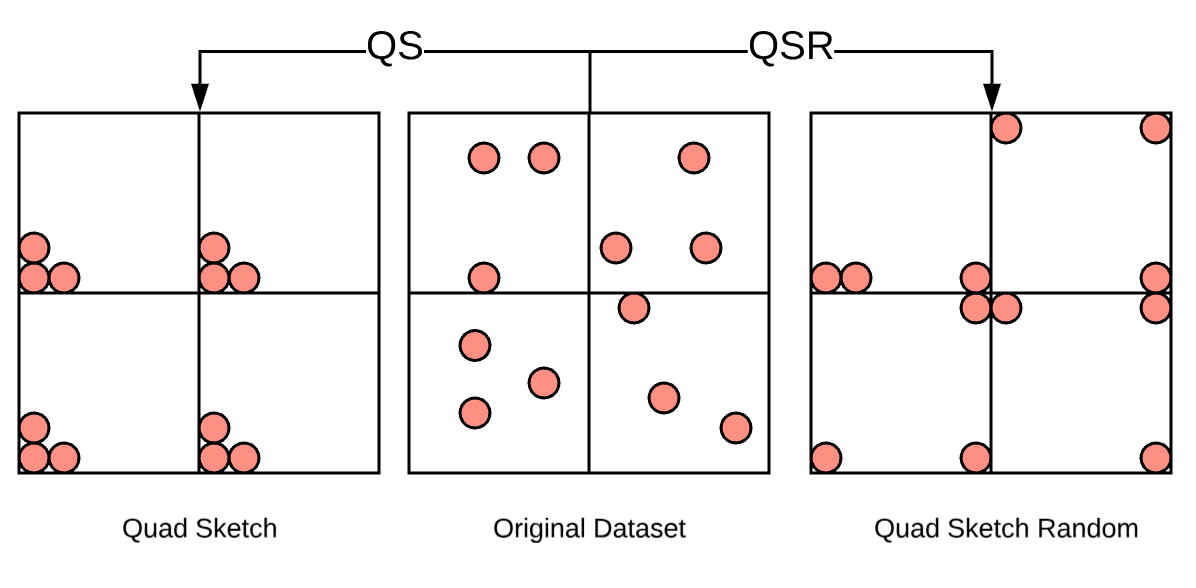
\includegraphics[width=1\textwidth]{figures/randombits}
	\caption{Random Bit Demonstration}
	\label{fig:randombits}
\end{figure}
The given example in figure \ref{fig:randombits} demonstrates a scenario where the experiment performs decently. It should be noted that the random movement of the points could also result in a worse representation. Such a scenario is discussed in \ref{disc/threats/randomness}.
\\
\\
The motivation of this experiment stems from the creation of the random quad tree in \qs{}. Should the creation of this \qt{} accidentally quad through closely clustered points then the distortion could be quite severe. By introducing randomness into the direction of the points, they might end up in corners closer to each other and thereby reduce the amount of distortion.
\section{Results}
\label{results}
%From ILO:
%"Plan and carry out a small-scale investigation of an algorithmic research problem. This investigation could be theoretical, experimental, or both."
This sections describes the results reached in the project. The goal in this section is threefold. Firstly to verify the results achieved in \cite{wagner17}. Secondly to explore the performance of \qs{} on new datasets. These datasets will have different properties than the datasets tested in \cite{wagner17}. Lastly to discover the performance of \qsr{} and compare this to the performance of \qs{}. 
\\
\\
The expirements are based on two datasets from the paper as well as two new datasets.\footnote{From \cite{wagner17} we use the datasets \sift{} and \mnist{}. Explicitly in this paper we have included \clust{} and \gist{}} For each dataset the results of \qs{} is verified and compared to the baseline implementation \gr{} and to \qsr{}. 
\\
\\
The results of these tests are illustrated as line charts. The charts visualizes the performance of the algorithms for each dataset measured in terms of \textit{accuracy pr bit of precision} and \textit{distortion pr bit of precision}. 
\\
\\
Similarly as in \cite{wagner17} the \qs{} implementations has been parameterized with \textit{L} ranging from 2 till 10 and $\Lambda$ ranging from \textit{L$_{min}$-1} to \textit{L$_{max}$-1}.\footnote{Their experiments range from \textit{L} ranging from 2 till 20 and $\Lambda$ 1 till 19. However the computation time for trees with a depth $>$ 14 is immense.} 
%\subsection{Practical improvements}
%Instead of randomly shifted ( works well for arbitrary, but maybe we know our data )
%On specific datasets:
%- Scale on spread out datasets, to avoid one point in each quad leaf
%- Zoom in on narrow / close datasets
\\
\\
The charts presented below displays results from the dataset\sift{}, \mnist{}. These results are key in verifying the results presented in \cite{wagner17}. Following this are the charts displaying results from \clust{} and \gist{}, as these disclose new information about the overall performance of \qs{}. Two graphs exists for each dataset displaying \textit{accuracy} and \textit{distortion} respectively. The graphs display that \qs{} has a better performance than \grid{} and verifies the results presented from empirical experiments in \cite{wagner17}.

\begin{figure}[h!]
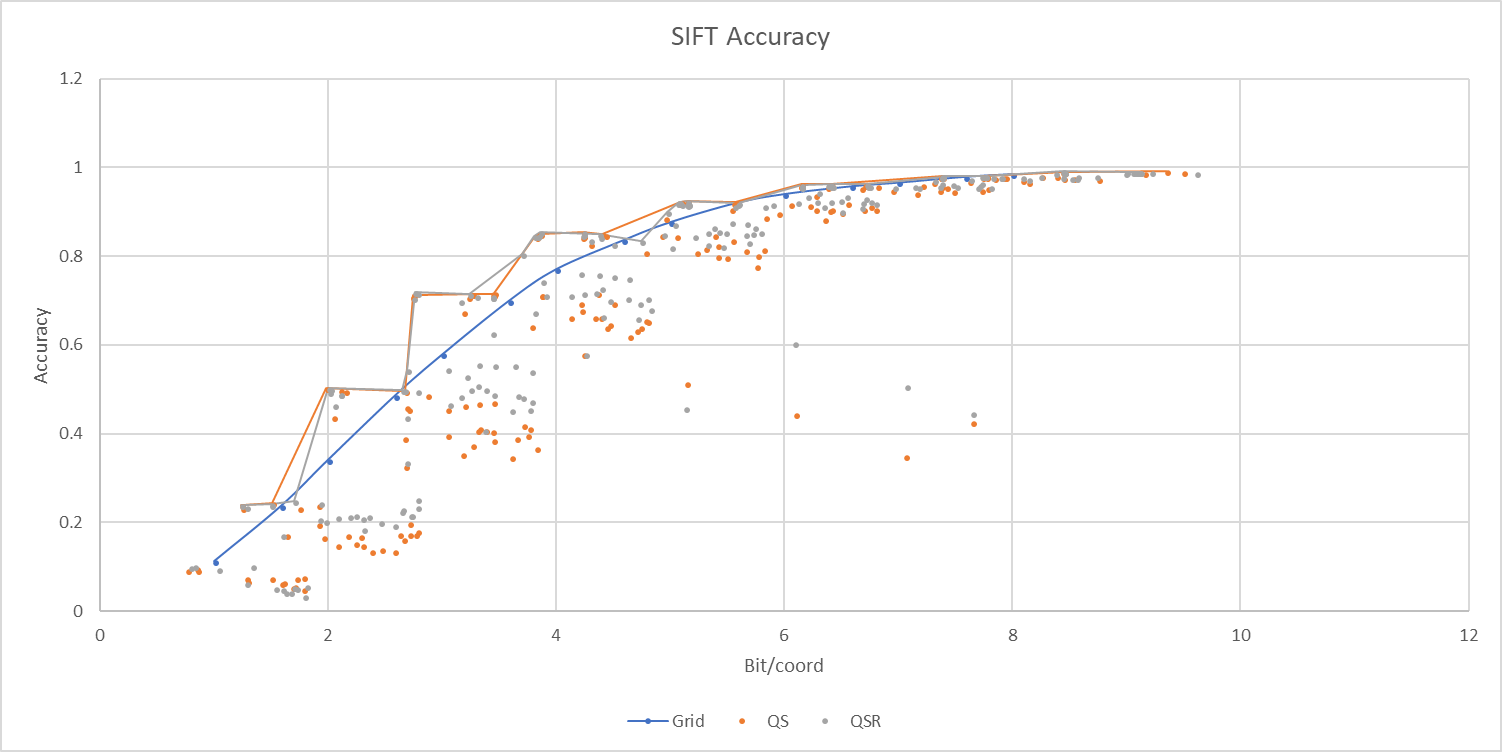
\includegraphics[width=\textwidth]{figures/graphs/sift_accuracy}
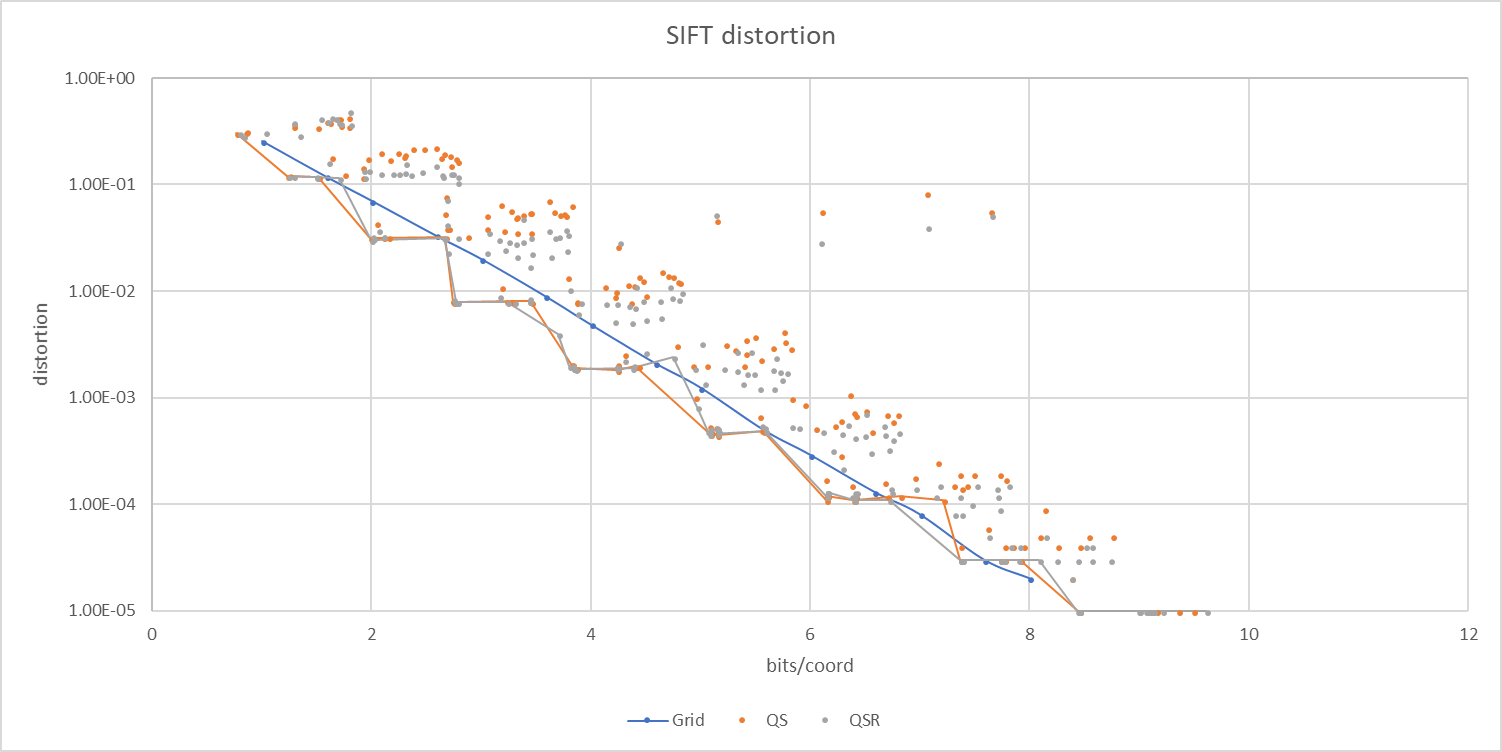
\includegraphics[width=\textwidth]{figures/graphs/sift_distortion}
\caption{Accuracy and distortion from \sift{}}
\label{fig:graph sift}
\end{figure}
The graphs in figure \ref{fig:graph sift} above show that in the best case scenario for \qs{} and \qsr{} are quite similar, while \qsr{} seems to be better in the average case.

\begin{figure}[h!]
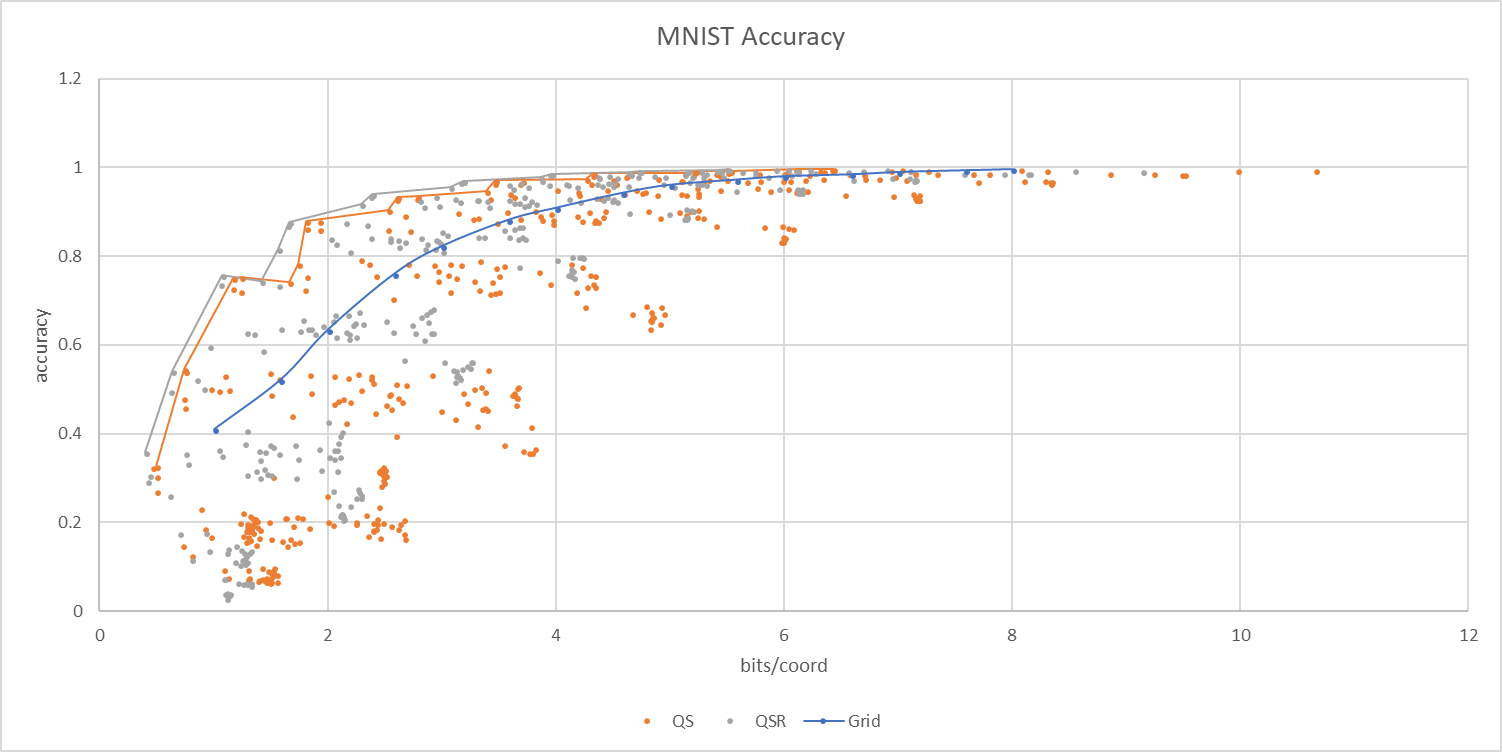
\includegraphics[width=\textwidth]{figures/graphs/mnist_accuracy}
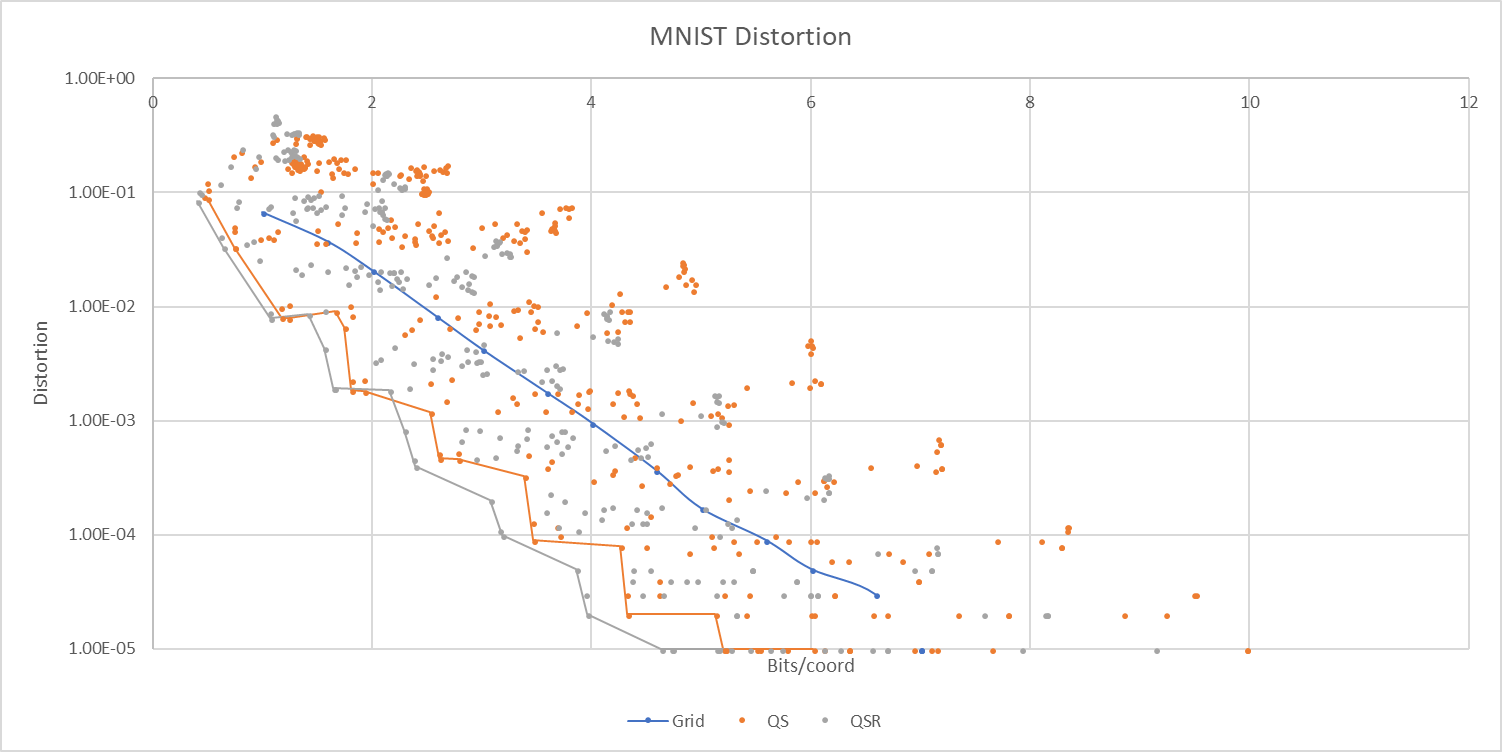
\includegraphics[width=\textwidth]{figures/graphs/mnist_distortion}
\caption{Accuracy and distortion from \mnist{}}
\label{fig:graph mnist}
\end{figure}
\clearpage
Figure \ref{fig:graph mnist} displays that \qsr{} runs are slightly superior to \qs{} in the best case regarding accuracy, and superior in regards to distortion. The average case for \qsr{} in distortion seems superior to the average case in \qs{}, but similar in regards to accuracy.

\begin{figure}[h!]
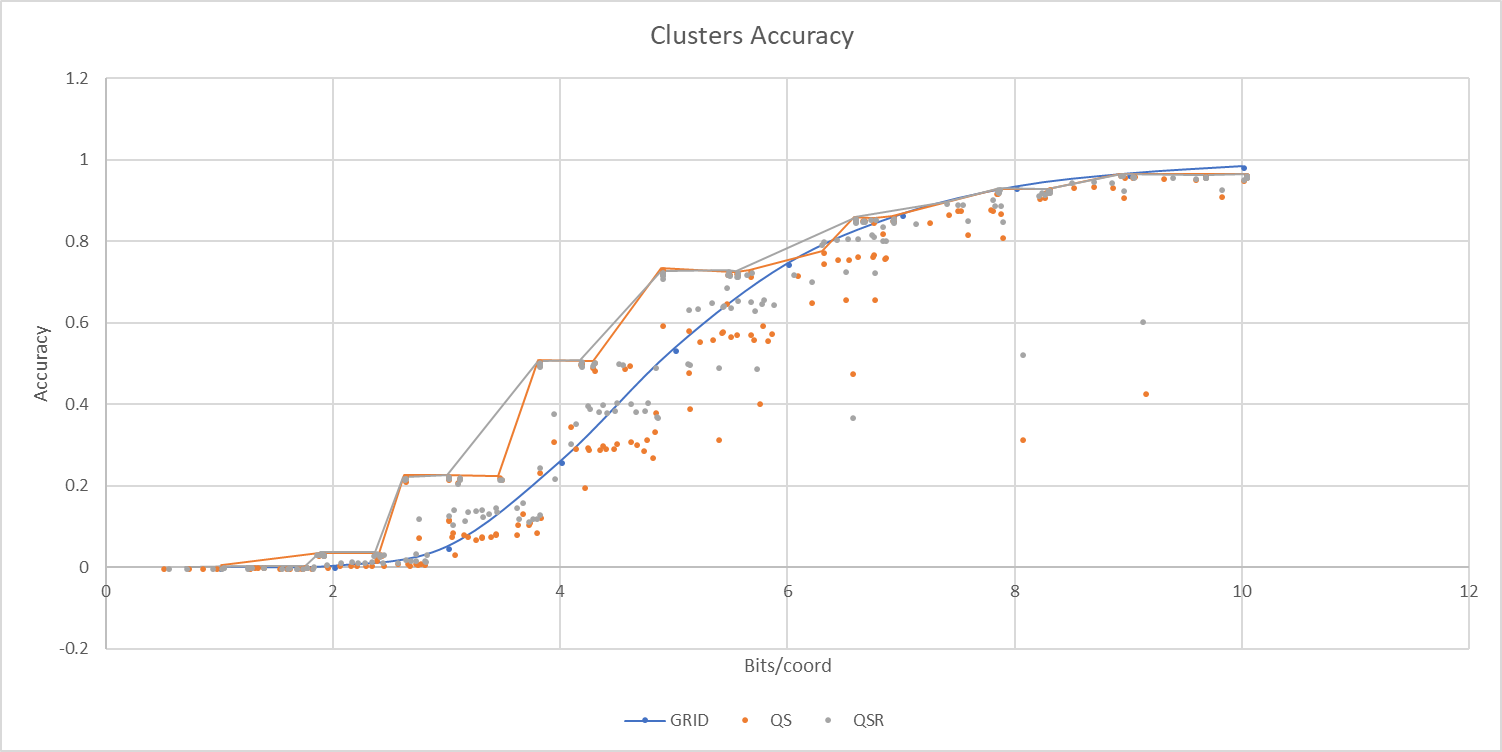
\includegraphics[width=\textwidth]{figures/graphs/clusters_accuracy}
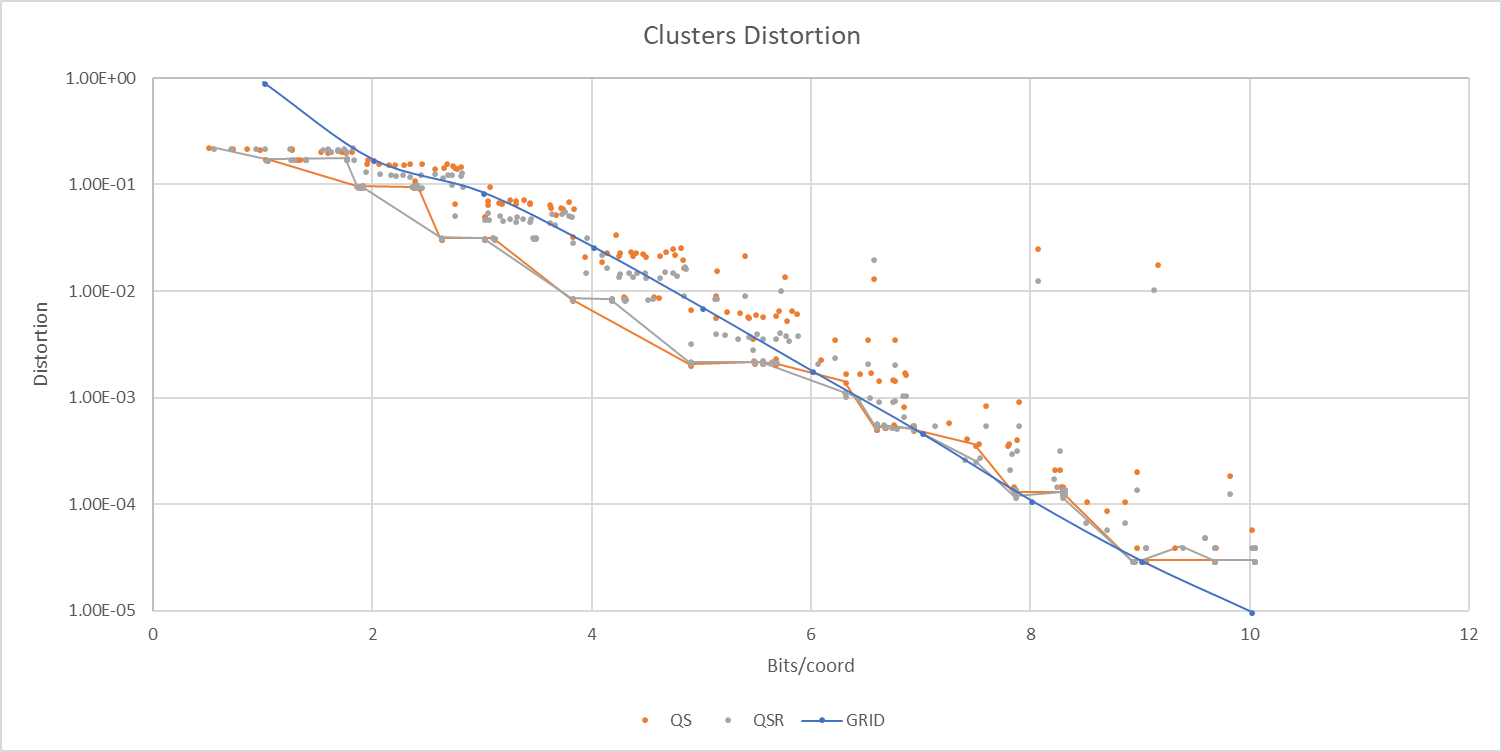
\includegraphics[width=\textwidth]{figures/graphs/clusters_distortion}
\caption{Accuracy and distortion from \clust{}}
\label{fig:graph clust}
\end{figure}
Figure \ref{fig:graph clust} shows that \qs{} and \qsr{} behaves similarly in best case runs for the clusters dataset. However the average case for \qsr{} is slightly superior to the \qs{} average results both regarding accuracy and distortion.
\clearpage{}

\begin{figure}[h]
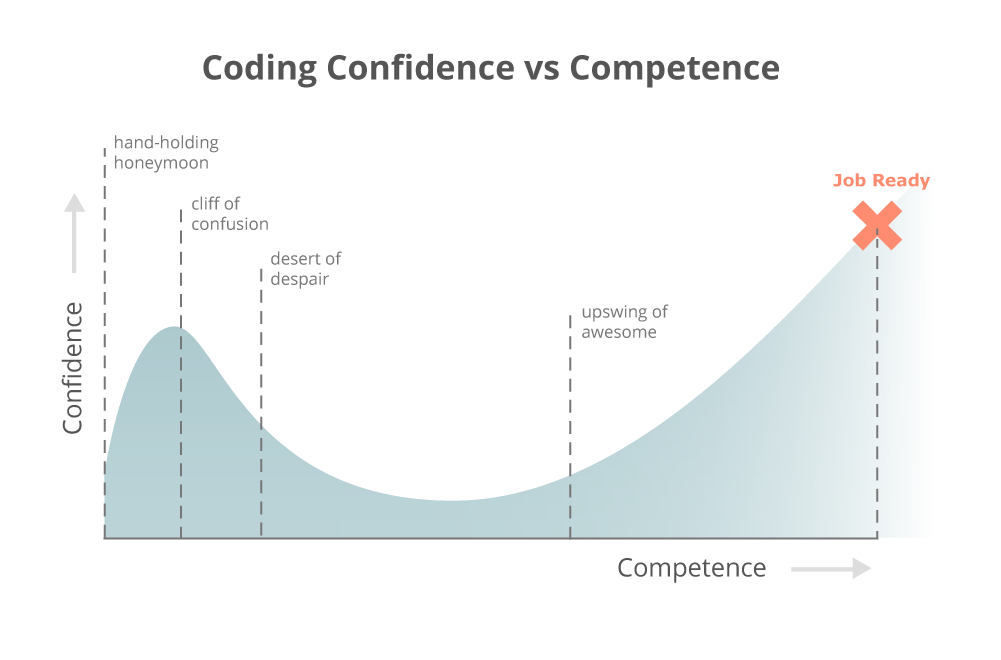
\includegraphics[width=0.5\textwidth]{figures/coding_graph}
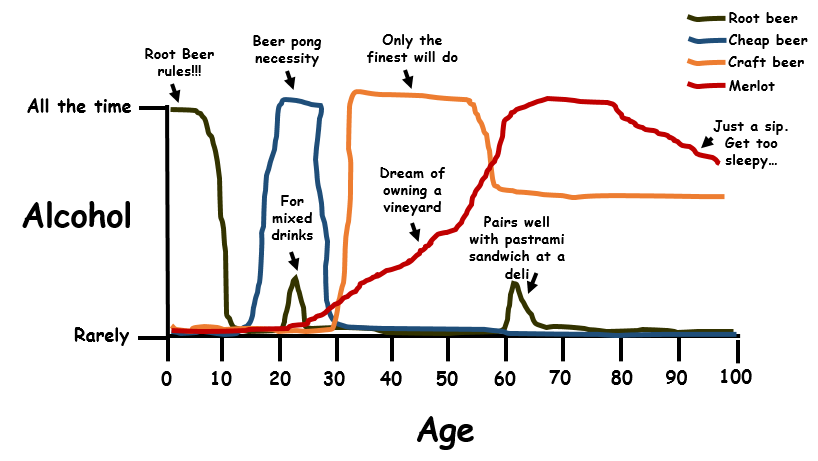
\includegraphics[width=0.5\textwidth]{figures/alcohol_graph}
\caption{Accuracy and distortion from \gist{}}
\label{fig:graph gist}
\end{figure}
Gist is the last dataset to demonstrate our extreme improvemnts. I am quite sure that we will impress Johan and Sam. And Erlich Bachmann (all heil). GG maybe this will not appear at all since the tests take a day to run each...


\section{Discussion}
\label{discussion}
This section discusses the findings presented in section \ref{results} and evaluates how the results relate to the goals stated in section \ref{intro:problemStatement}. Furthermore possible threats to validity of the results will be discussed.

\subsection{Verification of Performance}
The results in figures \ref{fig:graph sift} and \ref{fig:graph mnist} are used for verifying the results presented in \cite{wagner17}, where results showed that \qs{} outperforms the baseline \grid{} algorithm for the datasets \sift{} and \mnist{} in regards to both accuracy and distortion. In both figures it is clear that \qs{} indeed performs better than \grid{} and therefore confirms this trend. As the precise results in \cite{wagner17} have not been published, no distinct quantitative measure of the ‘similarity’ between the graphs have been used. It is not possible to get a precise reading of each node presented in the original graphs, and as such it is not possible to construct a similarity measure between any two nodes from the original graphs and the graphs created in this paper. 
\\
Apart from these obstacles, it is clear that the graphs are very similar, thus indicating that the results presented in \cite{wagner17} are accurate. It should be mentioned for clarity that outliers on the figures are the result of running \qs{} with inappropriate parameters e.g. there is pruned too much information. This process follows the original in \cite{wagner17}. These outliers help verify that the accuracy and distortion of the sketch is indeed controlled by the parameters \textit{L} and $\Lambda$.  

\subsection{Quadsketch and Quadsketch Random}
This subsection will focus on the comparison between \qs{} and \qsr{} as some interesting notions appear from the results. 
\\
Firstly both algorithms obtain approximately the same best scores for the datasets, except \mnist{} where \qsr{} achieves slightly better results. 
Secondly \qsr{} displays a better average case than \qs{} empirically (figures \ref{fig:graph sift}, \ref{fig:graph mnist} and \ref{fig:graph clust}), which aligns with the expectation from the theoritical improvements behind \qsr{}. The improvements are covered in section \ref{exp:dist}, where the random bit insertion in \qsr{} entails a lower expected distortion of the original pointset in regards to pruned points.
\\
The reason \qsr{} outperforms \qs{} on \mnist{} is due to the large amount of dimensions in the \mnist{} dataset. The more dimensions a dataset contains, the longer the bitstrings being pruned and replaced by quadsketch become. Longer bitstrings being replaced gives the random bit replacement a higher chance of converging towards the expected value. While the expected value grows whith the length of the bitstring, the lower expected value for \qsr{} bit replacement compared to \qs{} gives \qsr{} a better chance to get better accuracy and lower distortion. Even though the final result is data dependent, \qsr{} is likely to bring improvements over \qs{} on arbitrary highly dimensional data or cases where a lot of pruning is going to occur.

\subsection{Threats to validity}

\subsubsection{Randomness}
\label{disc/threats/randomness}
The comparison of the algorithms shown in \ref{results} show single test runs of the algorithms with different sets of parameters. The seemingly positive results for \qsr{} are inherently subdued to some randomness and could vary on further test runs. The same also applies to \qs{} as it makes use a randomly shifted grid, which also can effect on the outcome of single runs. \qsr{}'s added layer of randomness arguably facilitates the possibility of both worse and better outcomes than \qs{}.
%\subsubsection{Generated dataset}

\subsubsection{Depth of quad in experiments}
\label{disc/threats/depth}
In \cite{wagner17} the experiments on \qs{} and \grid{} runs the parameter $\Lambda$ 1 to 19 and \textit{L} 2 to 20. This project stops the $\Lambda$ at 9 and \textit{L} at 10 because the running time of \qs{} with larger parameters becomes infeasibly large for this project. As the results of this paper already discloses both accuracy and distortion values very close to one, the expected improvements gained by increasing the paramenters beyond the current bound are very limited. However it is possible that increasing the parameters would yield results that could disclose more information or other differences in the algorithms.

\subsubsection{Missing Dimensionality Reduction}
There is a slight offset between the results in \cite{wagner17} and the results in this paper. \cite{wagner17} uses Johnson-Lindenstrauss lemma to reduce the number of dimensions in a dataset to be $d=$\bo{$\epsilon^2\log(n)$}. A slight concern arises because it is unclear if the datasets \mnist{} and \sift{} used in this paper has been preprocessed with Johnson-Lindenstrauss. The concern derives from the \qs{} implementation provided on Github, because this implementation does not apply Johnson-Lindenstrauss as part of the source code. Therefore some investigation has been done in this area, and all though not confirmed it seems that the datasets have not undergone any preprocessing. A supportive argument entails that it would be natural to seperate these two processes, as this yields a more clean implementation of \qs{}. 
\\
In the given case that Johnson-Lindenstrauss has not been applied to the datasets, then the offset is natural (and should be expected), as the number of dimensions in a dataset has a direct impact on the number of bits required to represent a point. If this is not the case, then the results obtained in this paper disagrees with the results obtained in \cite{wagner17}. This is however deemed very unlikely. 
\section{Future Work}
\label{futurework}
This section will discuss what future work can be done as an extension to this paper and to \cite{wagner17}. Two new contributions will be shortly introduced and their main obstacles described. 

\subsection{Dynamic Addition}
Through the creation of this project some discussions has taken place regarding the possibilities of dynamically adding new points to the finished sketch without recomputing the entire datastructure. Computing the sketch is a very expensive operation, specifically for datasets with many dimensions and a high aspect ratio, as these require a larger tree to obtain propper metrics. This heavy compution currently limits the applications of \qs{} is therefore to static datasets. With the ability to dynamically add points would allow for further usages of \qs{}, and would therefore be a valuable contribution.  

\subsection{Automatic Parameters}

\section{Conclusion}
\label{conclusion}
Empirical experiments have verified the results found in \cite{wagner17} in regards to \qs{} on the included datesets\footnote{\mnist{} and \sift{}}. Furthermore the performance shown for \qs{} in the results holds for other datasets\footnote{\gist{} and \clust{}}.
\\
\\
A slight practical improvement to \qs{} in performance has been observed in empirical experiments using \qsr{}. The improvements are greatest on the dataset \mnist{}.



%\input{sections/title2.tex}
\clearpage

%bibliography
\bibliographystyle{apalike}
\bibliography{bibliography/references} 
\clearpage

%appendix
\appendix
%\section{Average results from experiments}
\label{app:a}
\begin{table}[h]
	\centering
	\caption{Average Results for \qs{} on \mnist{}}
	\label{table:avg_mnist_qs2}
	\begin{tabular}{l l l l}
		\hline
		\#Blocks & Bits per coordinate & Accuracy  & Distortion \\ \hline
		2 & 3.43 & 0.44 & 1.100  \\
		4 & 4.36 & 0.51 & 1.096  \\
		7 & 3.75 & 0.53 & 1.097 \\
		8 & 3.69 & 0.56 & 1.09 \\
		14 & 3.51 & 0.67 & 1.048 \\
		16 & 3.45 & 0.69 & 1.039 \\
		28 & 3.35 & 0.81 & 1.013 \\
		\hline
	\end{tabular}
\end{table}

\begin{table}[h]
	\centering
	\caption{Average Results for \qsr{} on  \mnist{}}
	\label{table:avg_mnist_qsr2}
	\begin{tabular}{l l l l}
		\hline
		\#Blocks & Bits per coordinate & Accuracy  & Distortion \\ \hline
		2 & 3.79 & 0.55 & 1.118  \\
		4 & 3.73 & 0.57 & 1.09  \\
		7 & 3.21 & 0.62 & 1.062 \\
		8 & 3.16 & 0.64 & 1.052 \\
		14 & 3.01 & 0.74 & 1.023 \\
		16 & 2.95 & 0.76 & 1.02 \\
		28 & 2.87 & 0.85 & 1.008 \\
		\hline
	\end{tabular}
\end{table}


\begin{table}[h!]
	\centering
	\caption{Average Results for \qs{} on \sift{}}
	\label{table:avg_sift_qs}
	\begin{tabular}{l l l l}
		\hline
		\#Blocks & Bits per coordinate & Accuracy  & Distortion \\ \hline
		2 & 4.32 & 0.49 & 1.122  \\
		4 & 4.64 & 0.61 & 1.056  \\
		8 & 4.39 & 0.7 & 1.034 \\
		16 & 5.15 & 0.85 & 1.008 \\
		32 & 5.68 & 0.78 & 1.025 \\
		\hline
	\end{tabular}
\end{table}

\begin{table}[h!]
	\centering
	\caption{Average Results for \qsr{} \sift{}}
	\label{table:avg_sift_qsr}
	\begin{tabular}{l l l l}
		\hline
		\#Blocks & Bits per coordinate & Accuracy  & Distortion \\ \hline
		2 & 4.33 & 0.52 & 1.112  \\
		4 & 4.63 & 0.65 & 1.04  \\
		8 & 5.02 & 0.77 & 1.018 \\
		16 & 5.44 & 0.83 & 1.015 \\
		32 & 5.68 & 0.79 & 1.02 \\
		\hline
	\end{tabular}
\end{table}

\begin{table}[h!]
	\centering
	\caption{Average Results for \qs{} \clust{}}
	\label{table:avg_clust_qs}	
	\begin{tabular}{l l l l}
		\hline
		\#Blocks & Bits per coordinate & Accuracy  & Distortion \\ \hline
		2 & 4.27	& 0.32 & 1.085  \\
		4 & 4.51 & 0.39 & 1.058  \\
		8 & 4.97 & 0.49 & 1.034 \\
		16 & 5.72 & 0.59 & 1.026 \\
		32 & 5.75 & 0.57 & 1.036 \\
		\hline
	\end{tabular}
\end{table}

\begin{table}[h!]
	\centering
	\caption{Average Results for \qsr{} on \clust{}}
	\label{table:avg_clust_qsr}
	\begin{tabular}{l l l l}
		\hline
		\#Blocks & Bits per coordinate & Accuracy  & Distortion \\ \hline
		2 & 4.26 & 0.33 & 1.08  \\
		4 & 4.5 & 0.42 & 1.048  \\
		8 & 4.97 & 0.52 & 1.03 \\
		16 & 5.72 & 0.61 & 1.025 \\
		32 & 6.08 & 0.63 & 1.026 \\
		\hline
	\end{tabular}
\end{table}

	
\end{document}